\documentclass[12pt]{article}

% Packages
\usepackage{amsmath}
\usepackage{amsfonts}
\usepackage{graphicx}
\usepackage{hyperref}
\usepackage{subfigure}
\usepackage[utf8]{inputenc}
\usepackage{appendix}
\usepackage{parskip}

\usepackage[backend=biber]{biblatex}
\addbibresource{references.bib}

% Graphics
\usepackage{tikz}
\usetikzlibrary{positioning, shapes.geometric}

% Title and Author
\title{A TypeScript based agent-based disease model}
\author{Heyan Zhu (Anson)\\
\footnotesize Mathmatics \& Computer Science Class\\
\footnotesize \texttt{heyan.zhu@ulink.cn}}
\date{\today}

\begin{document}

% Title Page
\maketitle

% Abstract
\begin{abstract}
This papers brings an agent-based model implemented by TypeScript, simulating the spread of diseases.
\end{abstract}

% \newpage
% Main content
\newcommand{\md}{\mathrm{d}}

\section{Introduction}
An agent-based model is a computer simulation of the interaction of agents (people) that is used to predict and demonstrate the spread of diseases. \textcite{columbiaGeneral}

\subsection{Math theory of spread of disease}
In the field of mathematics, there also exists a model known as the SIR model, which is a set of differential equations that describes the number of people who are susceptible ($S$, not infected), infected ($I$), and recovered ($R$, have recovered from the illness and are no longer susceptible to the same disease).
The equations of SIR model are as follows.

\begin{align}
    \frac{\md S}{\md t}&=-\beta S I\\
    \frac{\md I}{\md t}&=\beta S I-\gamma I\\
    \frac{\md R}{\md t}&=\gamma I
\end{align}

\begin{figure}[h]
	\begin{minipage}[h]{0.3\linewidth}
		\centering
		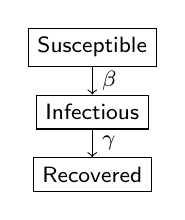
\begin{tikzpicture}[node distance=10pt]
    \tikzset{style={font=\sffamily\footnotesize}}
    \node[draw]                         (susceptible)   {Susceptible};
    \node[draw, below=of susceptible]    (infectious)    {Infectious};
    \node[draw, below=of infectious]     (recovered)     {Recovered};
    
    \draw[->] (susceptible)  -- node[right] {$\beta$} (infectious);
    \draw[->] (infectious) -- node[right] {$\gamma$} (recovered);
\end{tikzpicture}
        \caption{\scriptsize \sffamily The flow chart\textcite{mediumGeneral} of SIR model. }
	\end{minipage}
	\begin{minipage}[h]{0.7\linewidth}
		\centering
		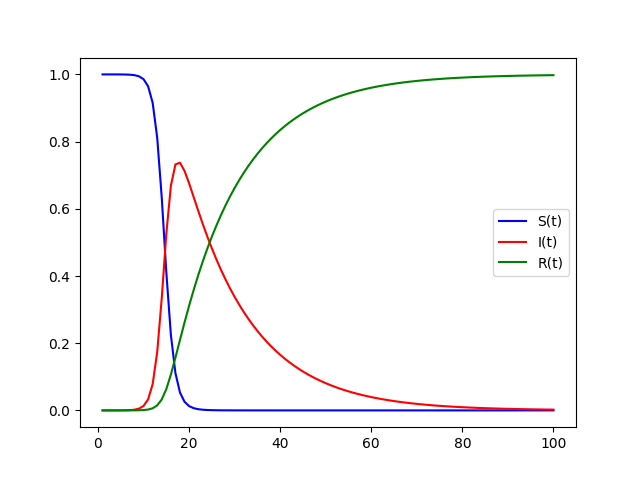
\includegraphics[width=\linewidth]{./assets/sir-graph.png}
         \caption{\scriptsize \sffamily The diagram\textcite{sirGraph} of SIR model. \\ \quad($\beta=1$ and $\gamma=0.1$)}
	\end{minipage}
	\label{fig:hor_2figs_1cap}
\end{figure}

% Methodology
\section{Methodology}

\subsection{Agent-based Model}
In order to construct an agent-based model, it is necessary to define the agents, their behaviours, the interactions between them, and the environment in which the agents operate. 
The agent-based model was implemented in TypeScript due to the author's familiarity with this programming language.
In general, agents are collections of properties, such as name, age, gender, health, and so on. They are used to represent the individuals, playing an important role in the simulation.
The behaviours of the agents in this model represent their daily routines and the locations of the agents at a specific time.

\subsection{Environment}
The environment can be defined as the space in which the agents reside. The dynamics of the agents can be understood as the movement of the agents within this space, which is influenced by their routines.

\subsection{Dynamics}
\subsubsection{Infection Possibility}
In order to simulate the spread of the disease, we need to consider how the healthy agents interact with the infected agents and get infected.
If the infected agents move close to the healthy agents, the risks of infection will be increased. A simple formulae which can roughly represent this is as follows.

\[
\mathbb{P}(\text{Infection})=\begin{cases}
	\dfrac{1}{d^2} &\quad \text{(for $d > 1$)} \\
	1 &\quad \text{(for $d \leq 1$)}
\end{cases}\quad\text{($d$ is the between the agents)}
\]

The graph of the above formula is shown in the figure below.

\begin{figure}[h]
	\centering
	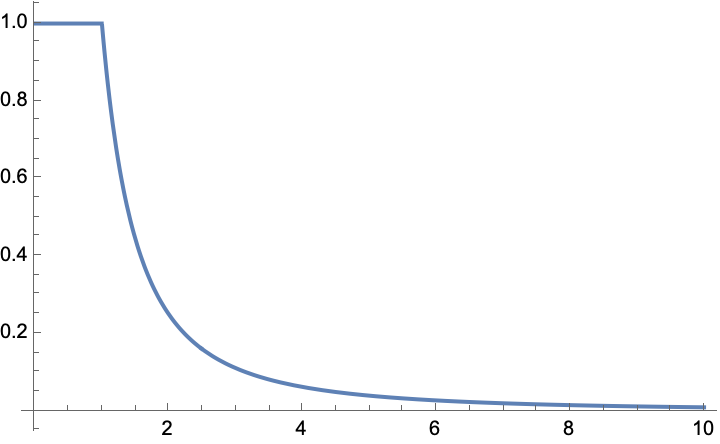
\includegraphics[width=0.7\linewidth]{./assets/infection-possibility-graph.png}
	\caption{The graph of possibility of infection.}
	\label{fig:infection-possibility-graph}
\end{figure}

Where the $x$ is the distance between the agents, calculated by the formula.

\[
d=\sqrt{(x_1-x_2)^2+(y_1-y_2)^2}
\]

Every agents will randomly get infected with a certain probability.

\subsubsection{Restoration}

As soon as the agents are infected, a timer will start to count down. When the timer reaches 0, the agents will be restored. The restored agents will not get infected by the same disease.

\subsection{Implemention}

In general, the model is implemented in TypeScript for the type safety which can structure the model well and make the code easier to understand, however, the graphing of the model is implemented in R, becuase of the powerful plotting package \texttt{ggplot2}.

The graph of the model \ref{fig:model-structure} which shows the design and the way that the modules cooperates with each other is shown in the appendix.

The flow chart of the model \ref{fig:model-flow-chart} is also placed in the appendix.

% Results
\section{Results}
The log of the model can be found in the appendix.
The result of the model is shown in the figure below. The parameters set in this model: 

\begin{itemize}
    \item Simulation Time: 60
    \item Agent Number: 40
    \item Room Size: 40
\end{itemize}

\leftline{The disease which in this simulation model:}

\begin{itemize}
	\item Disease Name: Cold
	\item Disease Severity: 100
	\item Disease Time to Restore: 10
\end{itemize}

\begin{figure}[ht]
	\centering
	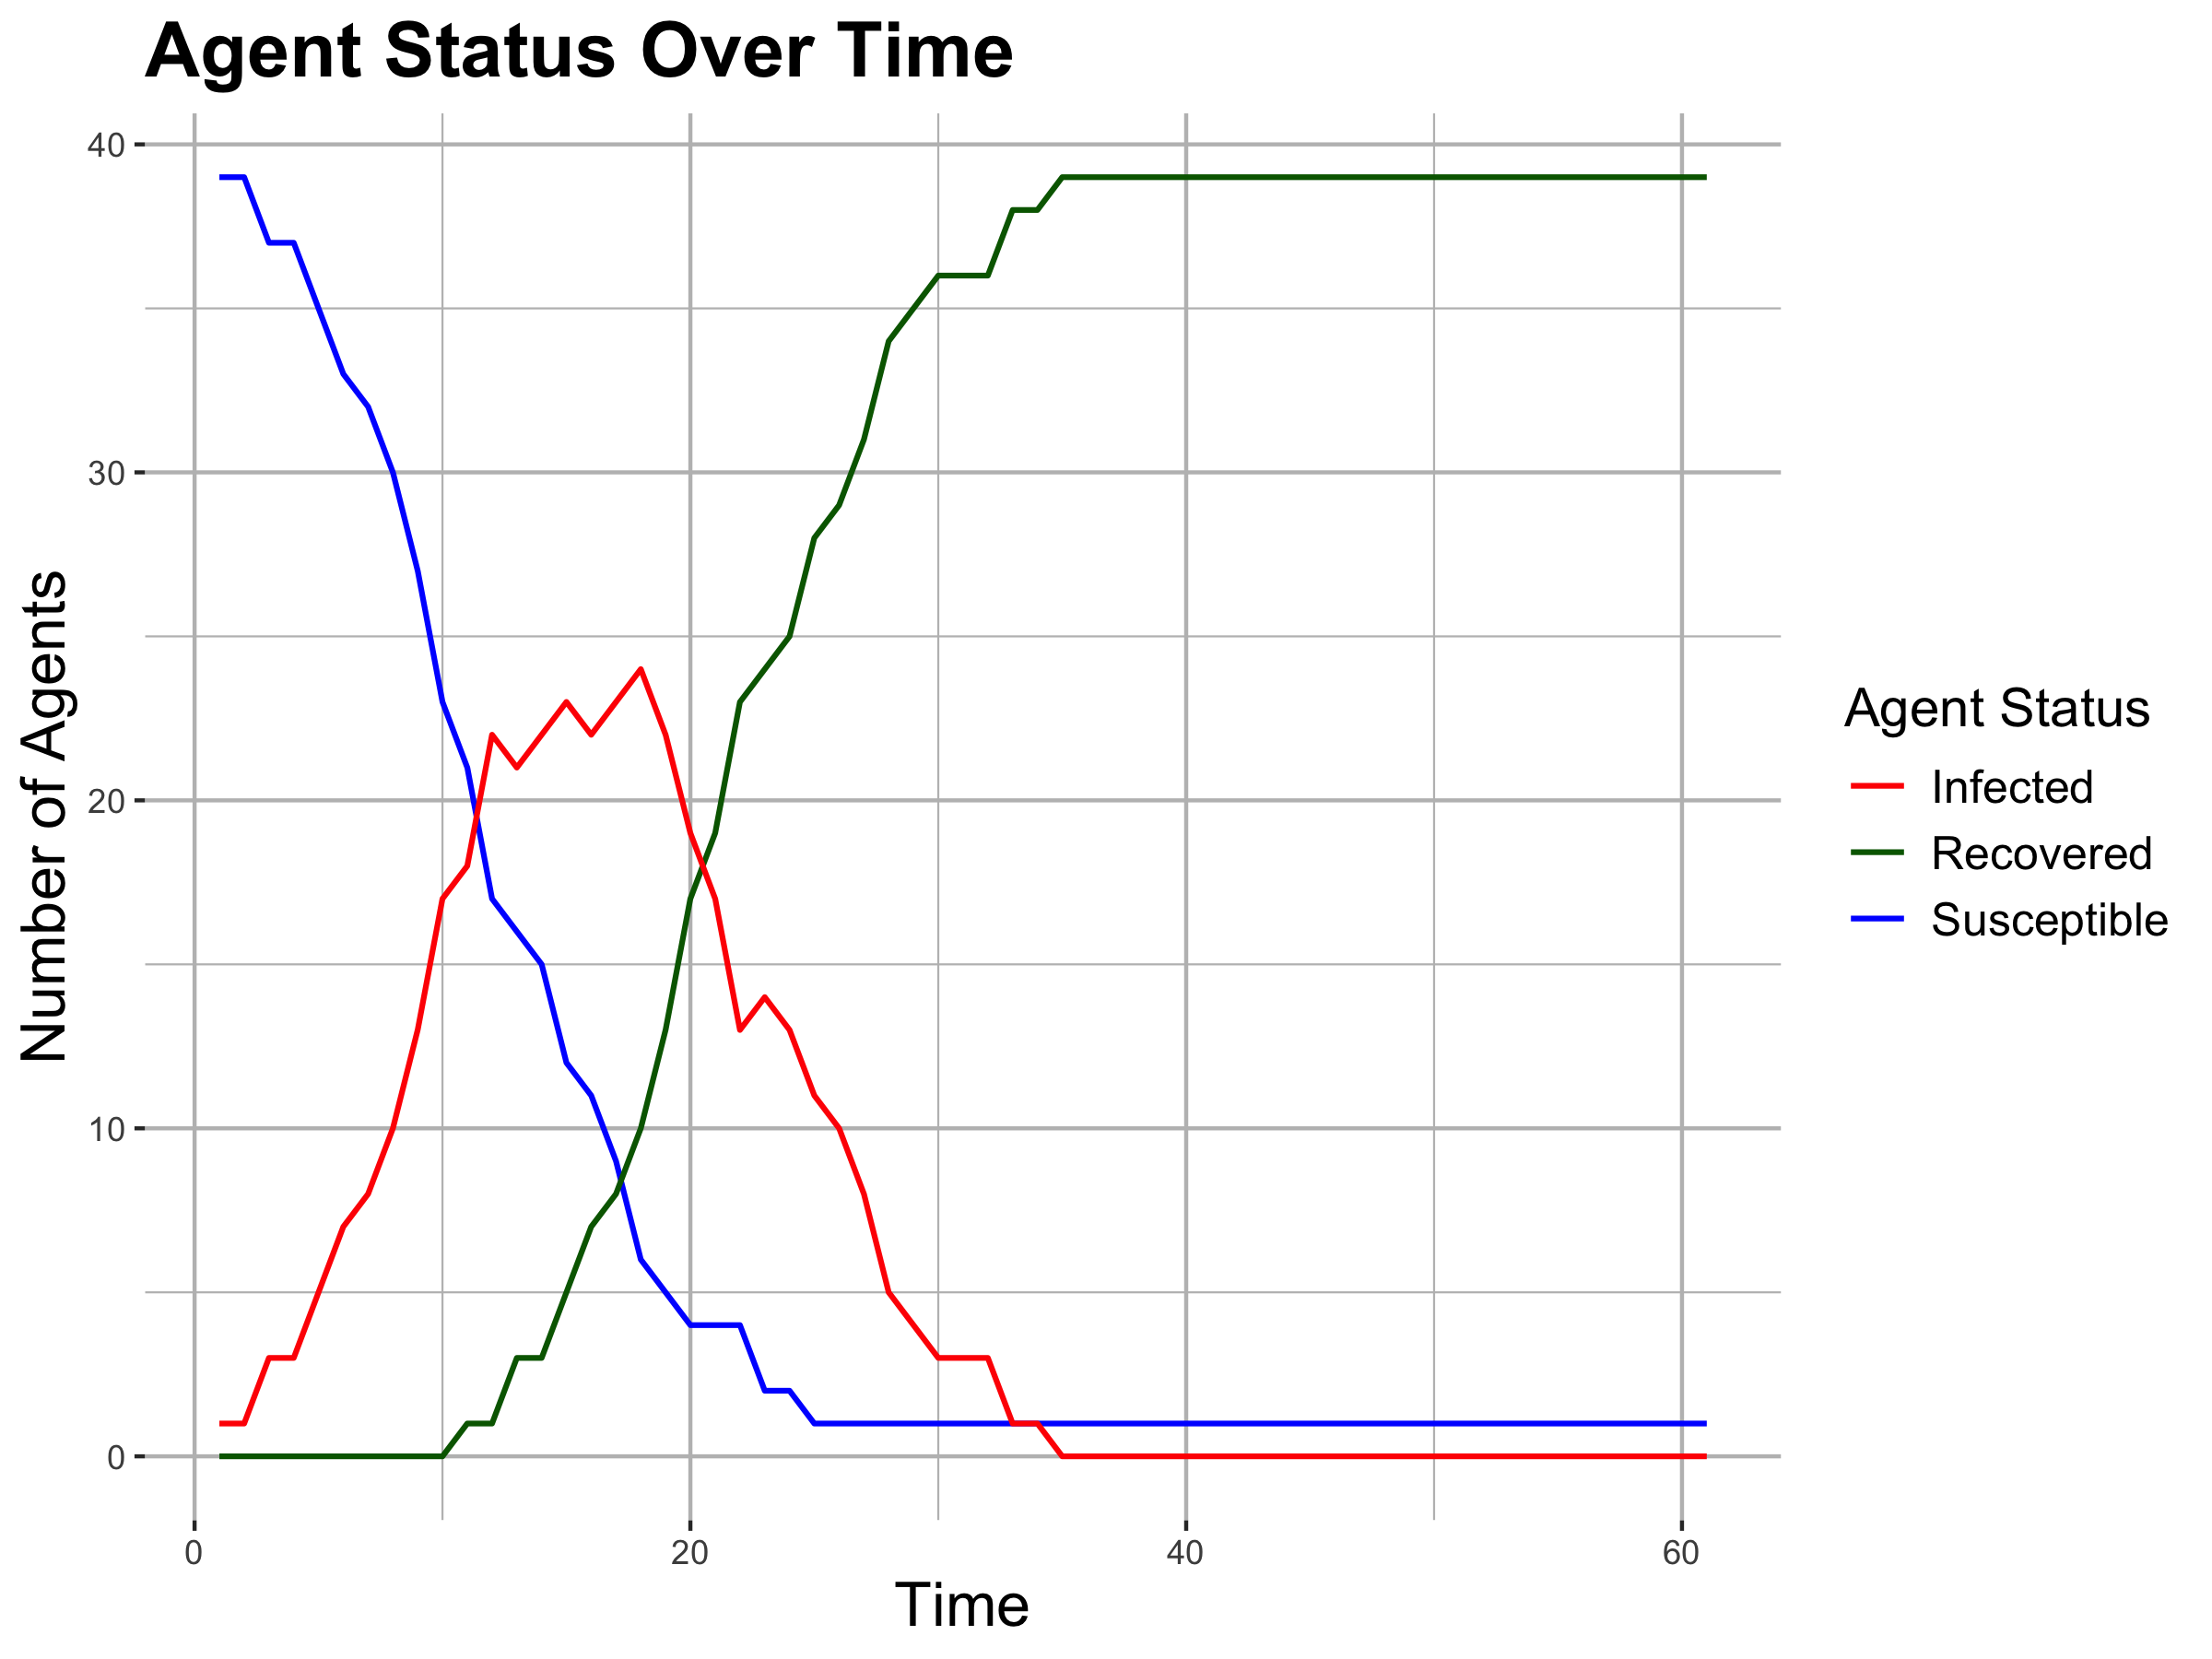
\includegraphics[width=0.9\linewidth]{./assets/report-20246030-132911/diagram.png}
	\caption{\scriptsize \sffamily The diagram of the created agent-based model}
\end{figure}

It is obvious that this model can partially simulate the spread of the disease with given parameters with the agents and diseases, because of the similiarty between Figure 2 and Figure 4 with the outbreaks and extinctions.

% Discussion
\section{Discussion}
This model is a good model to simulate the simple spread of the disease, written in TypeScript, for the sake of simplicity, but lack of ability to simulate the multiple diseases with complex dynamics.
Some feature that can migrate and control the parameters of $\beta$ and $\gamma$ are missing, should be added in the future.
Becuase of the familiarity of the TypeScript, author choose to write in this language, which is not common for the data analysis. It can be better if the model can be implemented with Python or R.

% Conclusion
\section{Conclusion}
The above model can successfully simulate the spread of the disease, with the outbreak and extinctions.

% References
\section{References}
\printbibliography[heading=none]

\newpage

\section{Appendix}
\begin{appendices}
    \subsection{The log of the agent-based model}
    The log for the run from the model can be found in this URL. \url{https://pastecode.io/s/jb6npovz}. The routine of the agent has been set to randomly move.

    \newpage

    \subsection{The structrue of the agent-based model}
    \begin{figure}[ht]
		\centering
		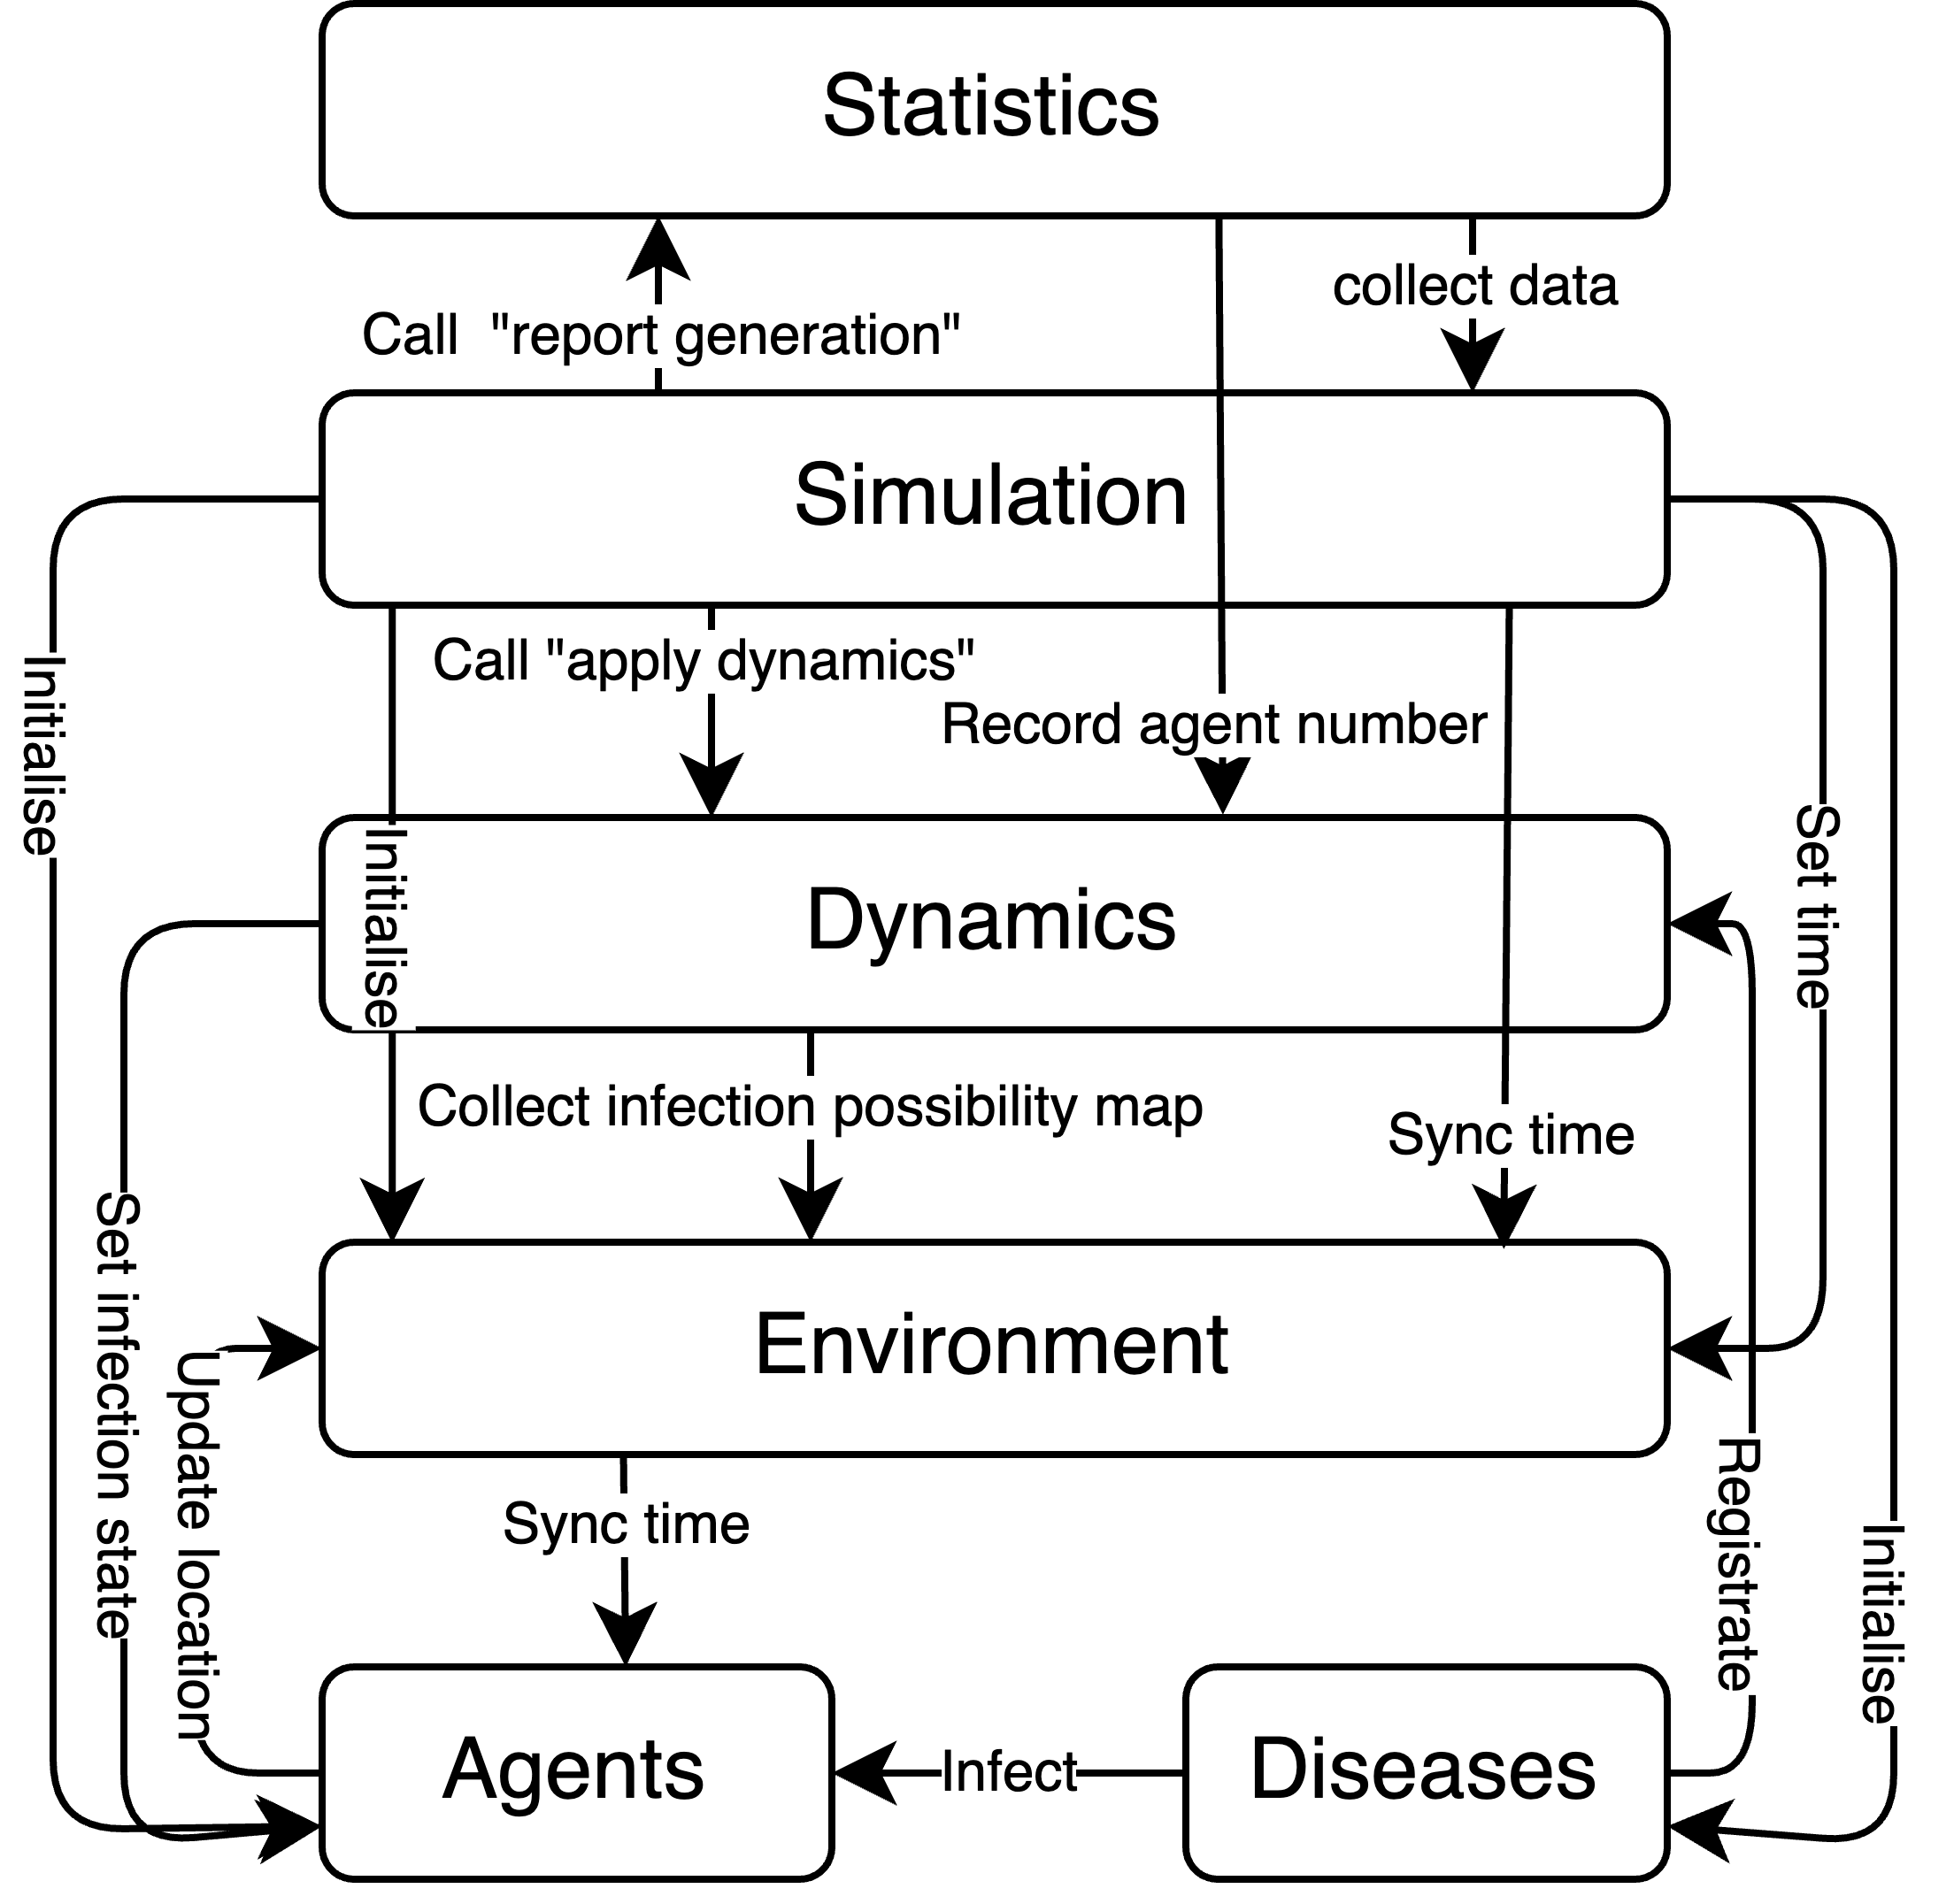
\includegraphics[width=0.6\linewidth]{./assets/model-structure.png}
        \label{fig:model-structure}
		\caption{\scriptsize \sffamily The structure of the created agent-based model} 
	\end{figure}

    \newpage

	\subsection{The flow chart of the agent-based model}
	\begin{figure}[ht]
		\centering
		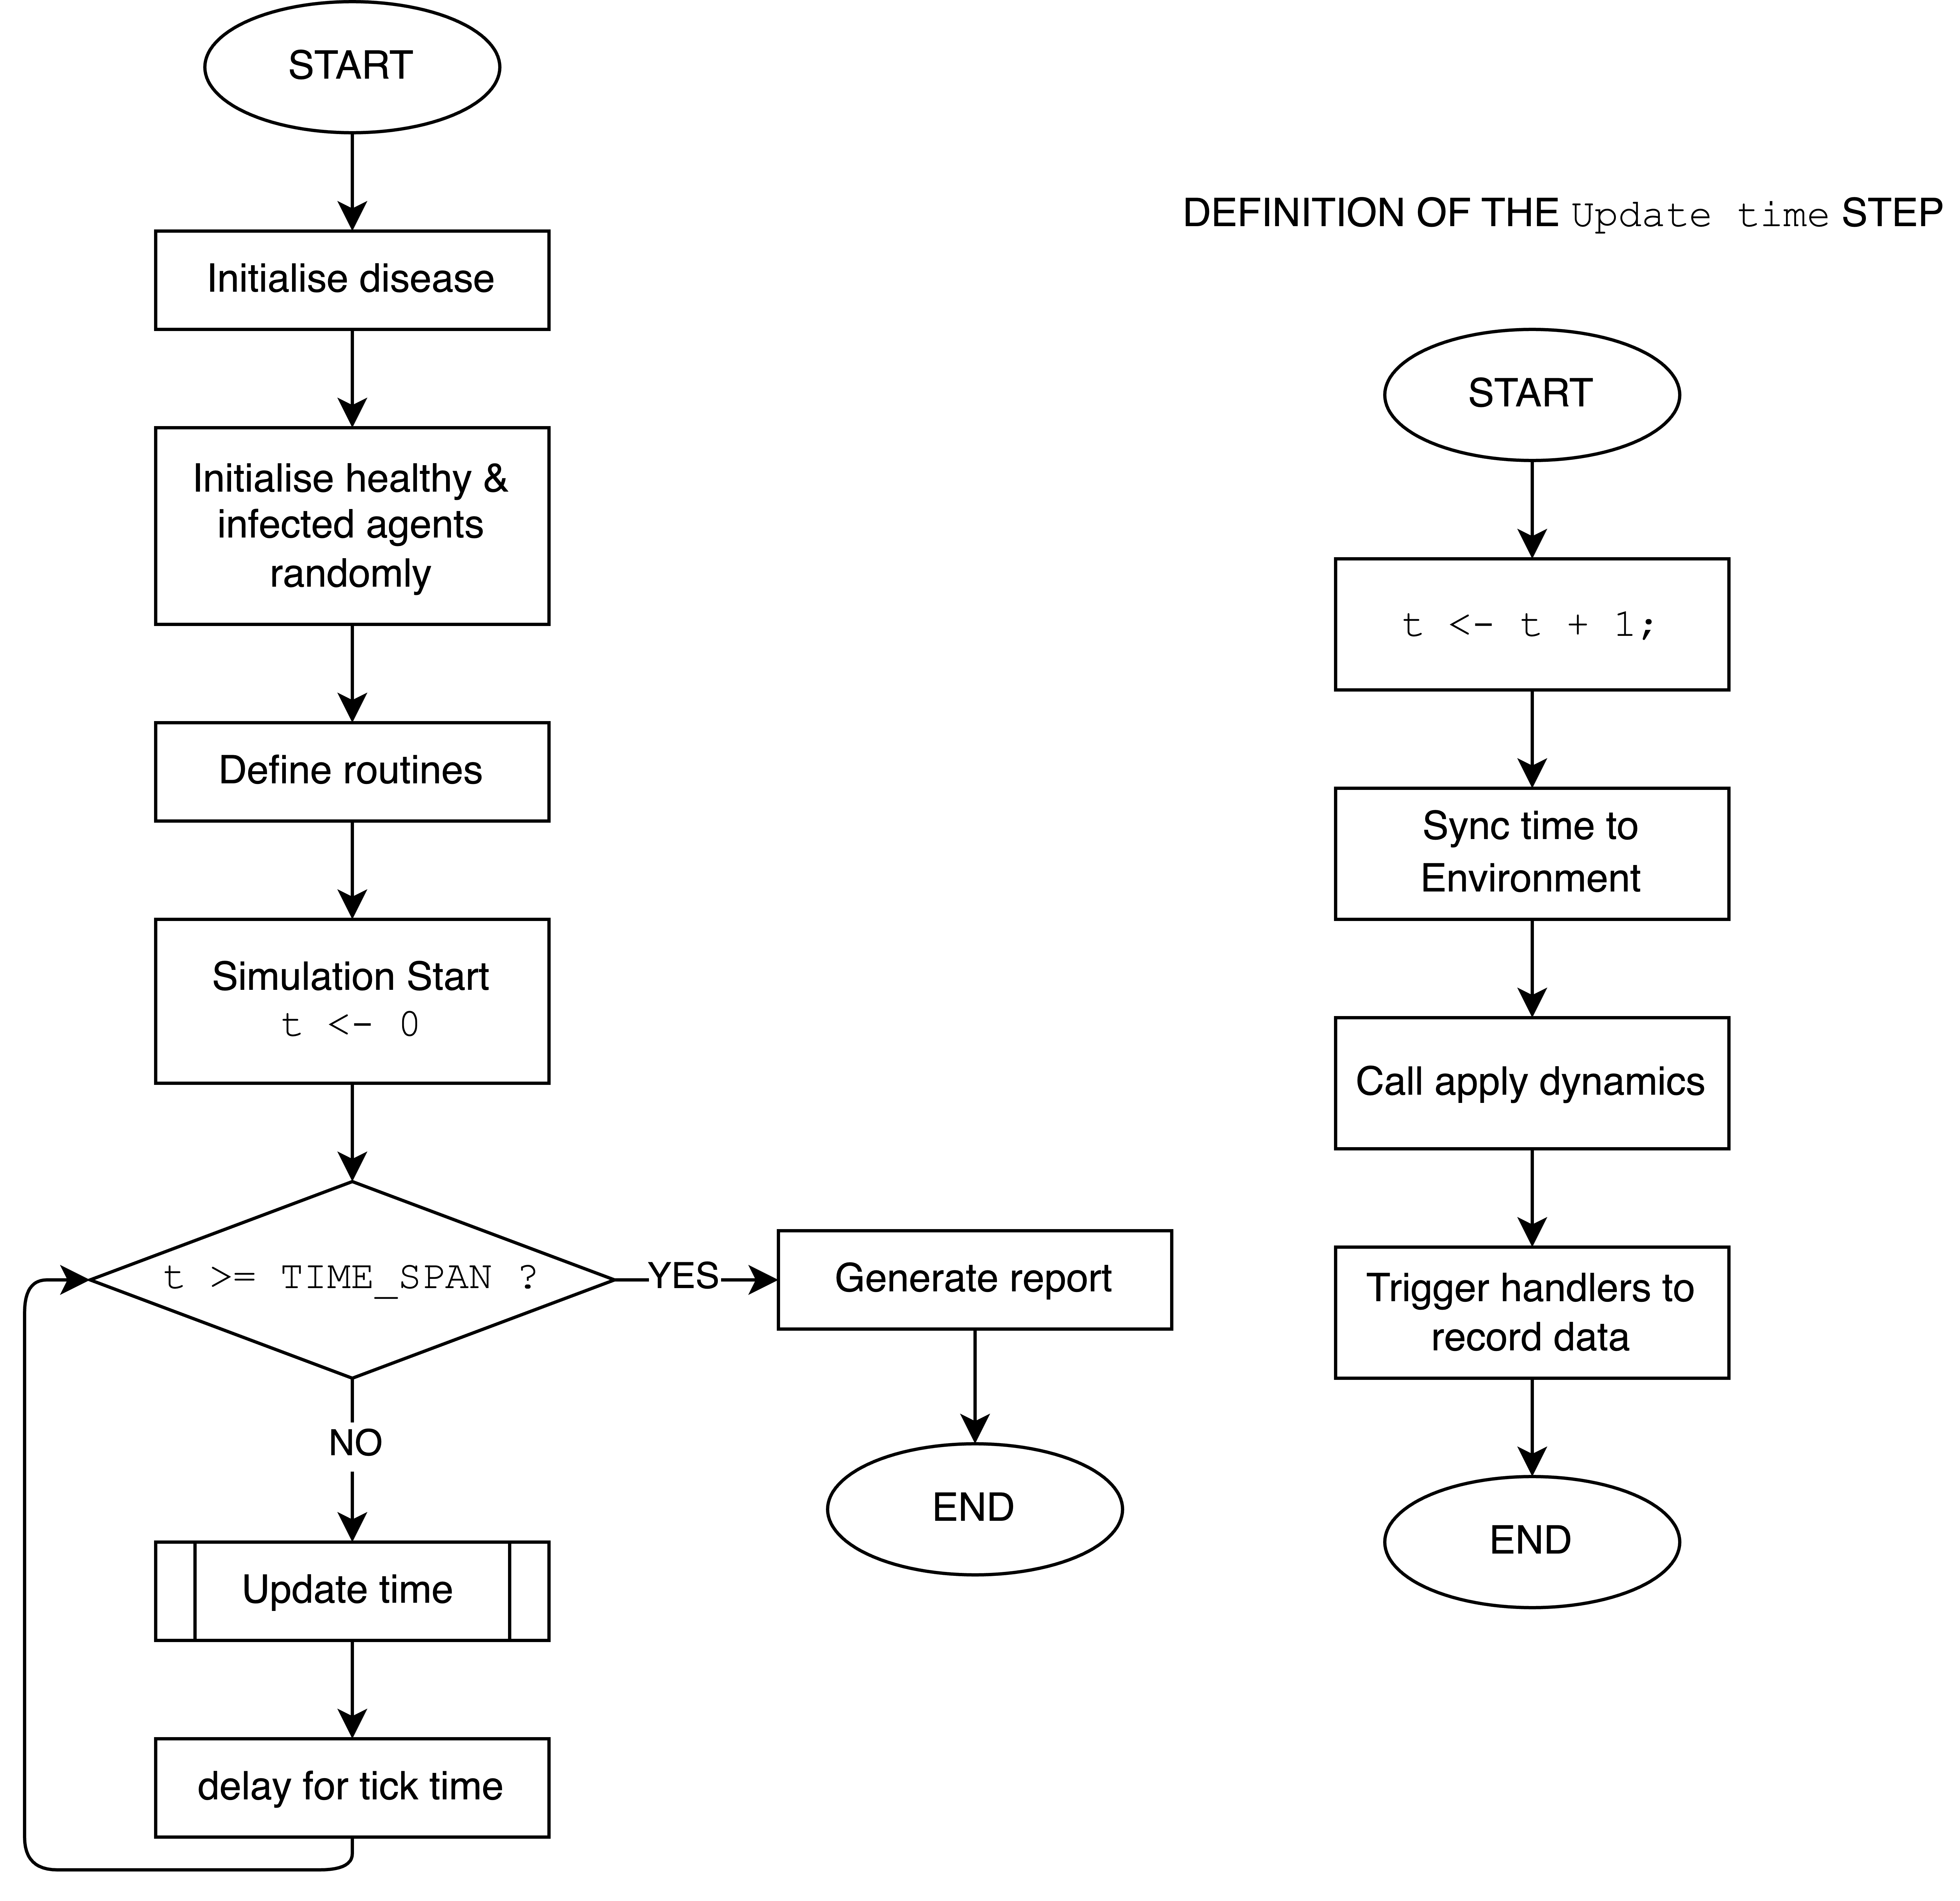
\includegraphics[width=\linewidth]{./assets/model-flow-chart.png}
        \label{fig:model-flow-chart} 
		\caption{\scriptsize \sffamily The flow chart of the created agent-based model}
	\end{figure}
\end{appendices}

\end{document}